\section{Massively Learning Activities I - Initial Deployment} \label{section: MLA}

Although project development plans can differ, they commonly follow a similar framework known as the SDLC (System Development Life Cycle). The System Development Life-cycle (SDLC) is a project management model that defines different stages that are necessary to bring a project from conception to deployment and later maintenance. 

The SDLC model consists of several phases: planning, research, design, implementation, testing \& integration, and maintenance. It provides a systematic approach to system development that helps ensure that system is built efficiently with minimal risk.

We explore the logistics of configuring a multi-tenant environment by documenting the entire project management process, inspired by the System Development Life-Cycle framework.  Massively Learning Activities will follow a similar variation of the SDLC project management model where each SDLC stage will correspond to a subsection in this chapter. 

\begin{figure}[H]
    \centering
    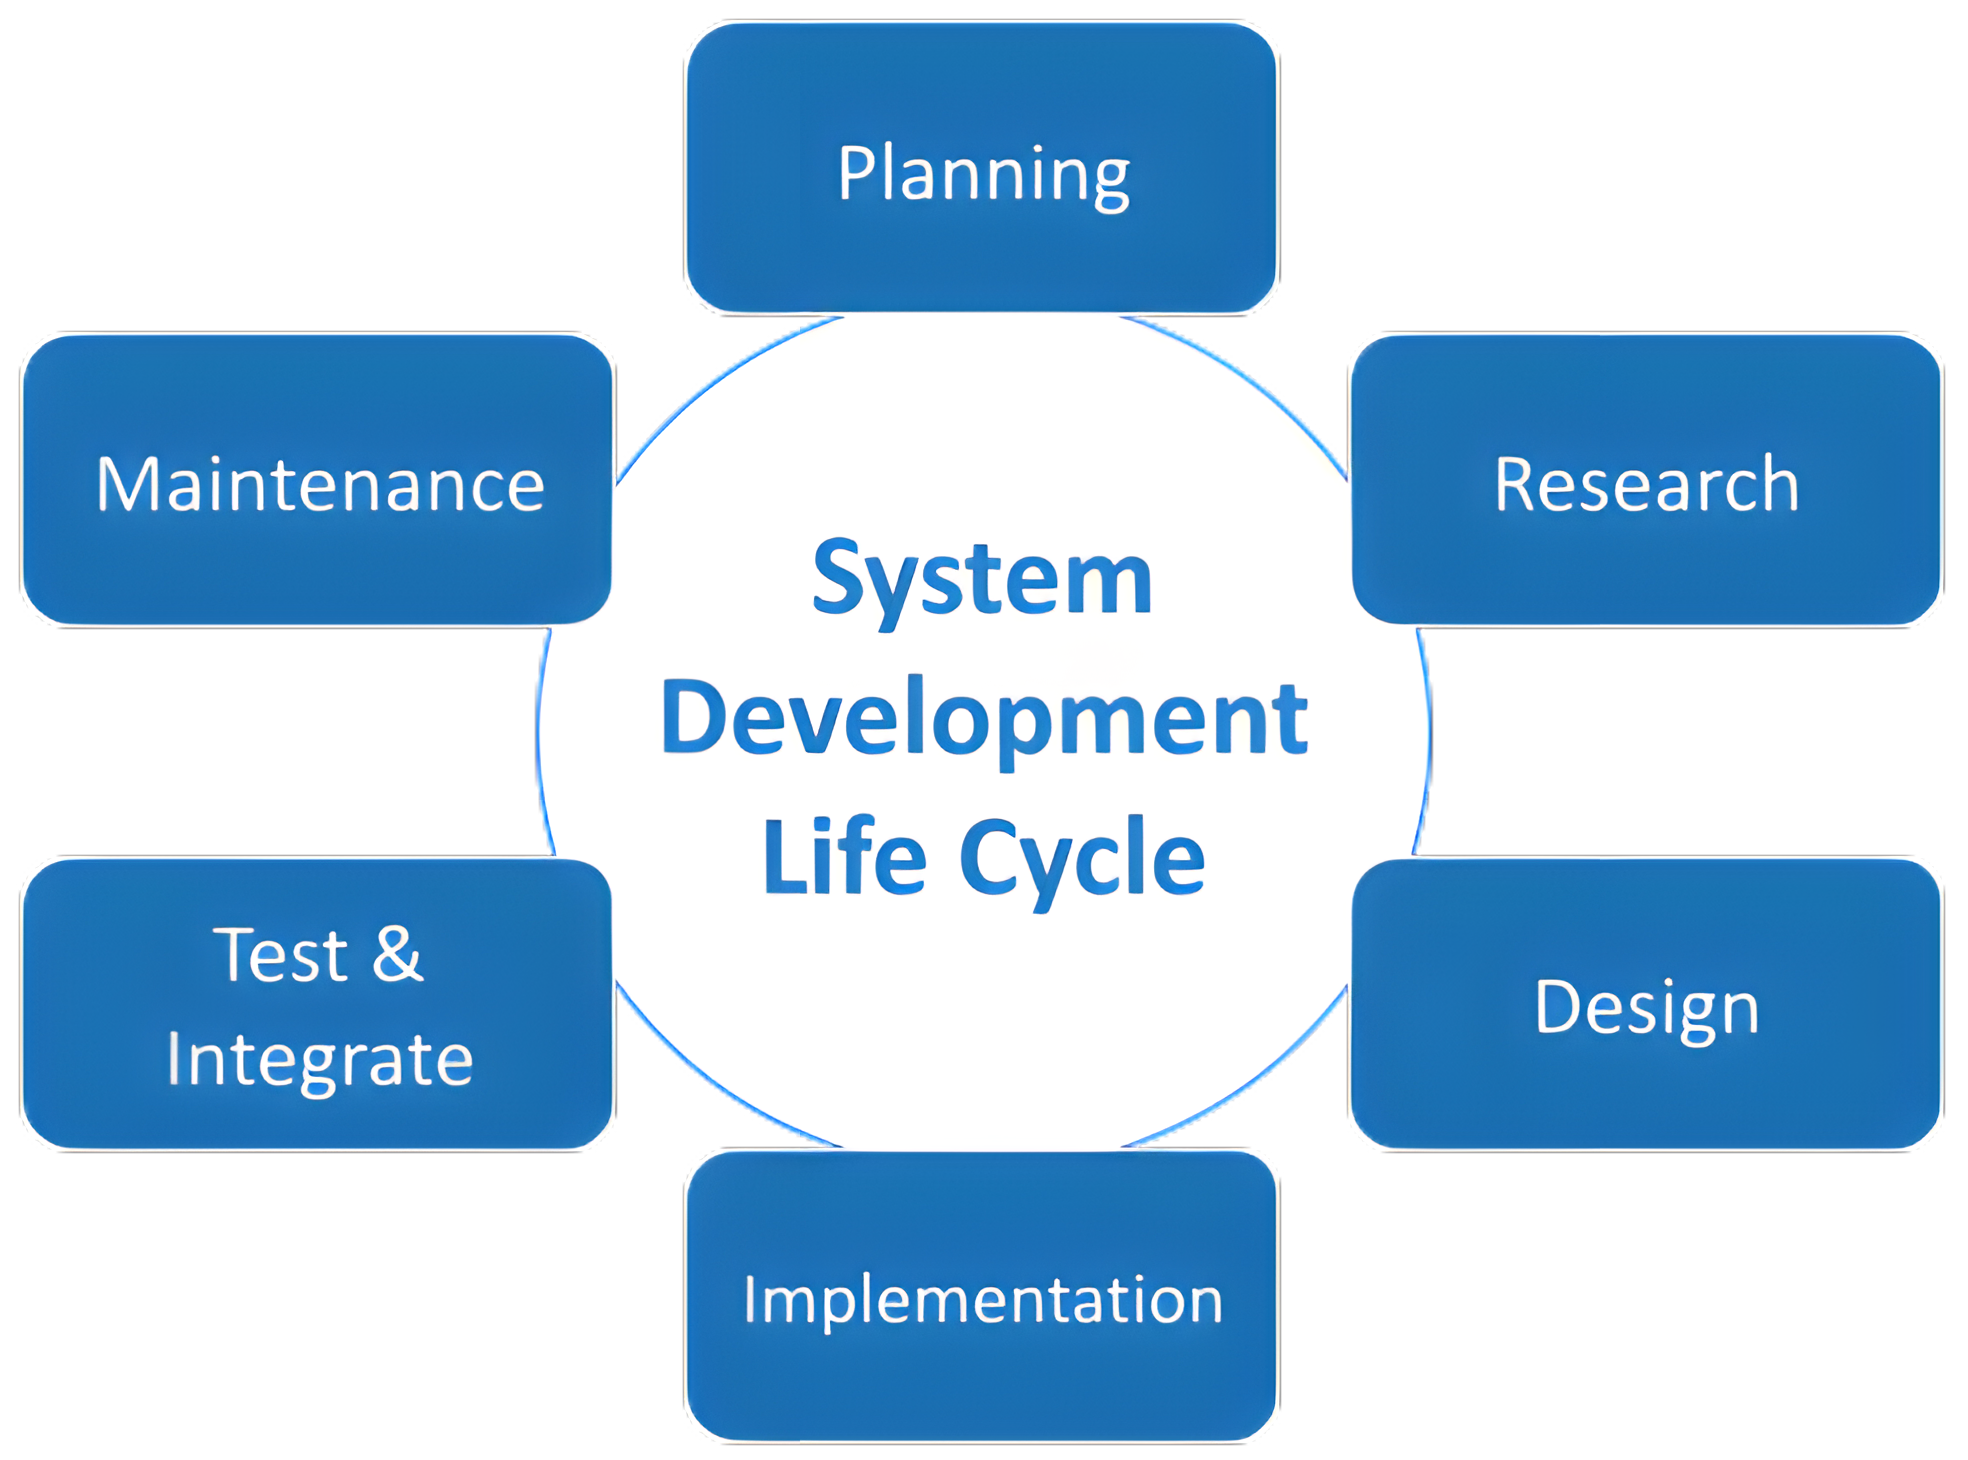
\includegraphics[scale = 0.175]{images/SDLC.png}
    \caption{System Development Life-Cycle}
    \label{SDLC}
\end{figure} 

%----------------------------------------------------------------------------------%

\subsection{Planning I} 

TASI has been contracted by CNMI to create an infrastructure that will allow for data analytics on Protected Health Information (PHI). To achieve this, TASI will provide a Platform as a Service (PaaS) solution, by hosting SAS services on on-premises hardware, configured for multi-tenancy.

Tenants will provide the data, which will be submitted through an ETL pipeline for data migration, cleaning, and processing. Once the data has been processed, tenants may perform data analytics using advanced algorithms in SAS programming language.

Due to SAS being a time sensitive project, the initial deployment will have SAS suites and VMs installed on existing hardware, with plans to migrate the infrastructure to newly acquired hardware in the future.

MLA I will expect 4 tenants:
\begin{enumerate}
    \item Commonwealth of the Northern Mariana Islands (CNMI)
    \item All-Payer Claims Database (APCD)
    \item Centers for Medicare \& Medicaid Services (CMA)
    \item Med-Quest
\end{enumerate}

\subsection{Requirement of Analysis I}

The Requirement Analysis phase is a crucial component in developing a robust SAS infrastructure using the SDLC framework. This phase involves gathering and analyzing the specific requirements for the project, including pre-installation checklists and EEC sizing requirements. In this phase, ongoing project management tasks will be performed, such as preparing a project plan and assigning appropriate resources. 

Furthermore, as part of this phase, SAS will send a Pre-Install Requirements Document to the client for completion, and both parties will ensure environmental readiness for installation by reviewing the completed document. 

Additionally, SAS will send a billable work hours log for verification based on the project plan. This subsection will provide a detailed overview of the pre-installation checklist and EEC sizing requirements necessary for a successful implementation of the SAS infrastructure.

\subsubsection{TASI's Infrastructure}
\label{TASI's Infrastructure Section Header}

The internal infrastructure of UHTASI is designed to ensure secure and efficient environment. The process begins with an internet connection, which is routed through the UH internet. To protect the network, we have implemented both a North/South (N/S) firewall and an East/West (E/W) firewall, which serve as barriers against unauthorized access and help to safeguard our data.

For enhanced reliability, redundancy is a key aspect of our infrastructure. We have two network switches in place, ensuring that if one switch fails, the other seamlessly takes over to maintain uninterrupted connectivity.

At the core of our infrastructure, we have a Dell FX2 Enclosure. The FX2 Enclosure is a 2U rack-based server located inside a server rack at the ITS data center (ITS M01). There are four blade servers that exist within the enclosure. Each blade is a self-contained server that contains one or more CPUs, memory, storage, and other components required to run applications and services. The ITS data center ensures a high level of reliability with a guaranteed 99.8\% availability of network, power, and cooling components as stated in the service level agreement (\href{https://www.hawaii.edu/its/docs/CoLocationSLA.pdf}{SLA}).

To facilitate data storage and retrieval, we have incorporated two SAN (Storage Area Network) network switches for redundancy. These switches provide a dedicated network infrastructure for our storage, ensuring fast and reliable access. In addition, UHTASI has installed an expansion slot on the SAN to increase the overall capacity of the SAN's storage. The connection between the network and SAN switches and the Dell FX2 Enclosure is a 10-gigabit link.

\begin{figure}[H]
    \centering
    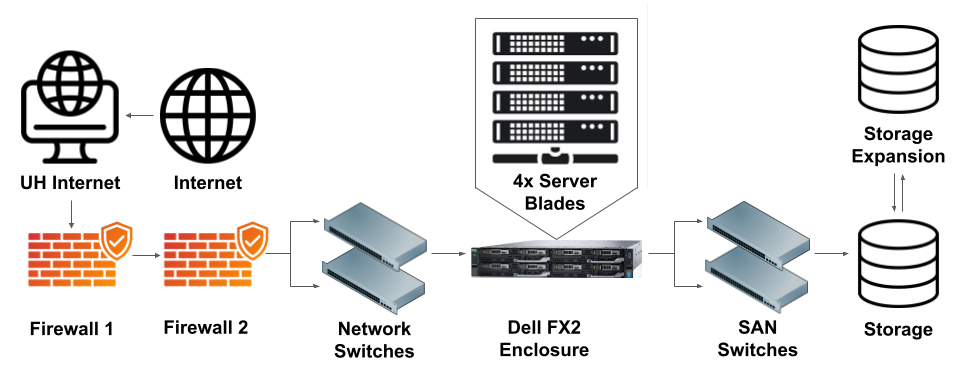
\includegraphics[scale = 0.64]{images/UHTASI Infrastructure.png}
    \caption{UHTASI On-Premise Infrastructure}
    \label{UHTASI-INF}
\end{figure}

Despite each blade in the FX2 Enclosure already being allocated to other TASI projects, the unused resources will be logically separated to establish a multi-tenant environment that can facilitate SAS technologies.

\newpage 

\subsubsection{Multi-Tenancy Configuration Plan: VM Location}
\label{Multi-Tenancy Configuration Plan}

\begin{figure}[H]
\begin{center}
    \renewcommand{\arraystretch}{1.5}
    \begin{tabular}{|>{\raggedright\arraybackslash}l 
                    |>{\raggedright\arraybackslash}m{6cm} 
                    |>{\raggedright\arraybackslash}l 
                    |>{\raggedright\arraybackslash}l 
                    |}
    \hline
    \rowcolor[HTML]{196fb4}\centering\textcolor{white}{\large Server Name} 
                            & \centering\textcolor{white}{\large Function}  
                            & \centering\textcolor{white}{\large Site} 
                            & \centering\textcolor{white}{\large Physical Server} 
                            \tabularnewline 
    \hline
    DC1	           & LDAP Host1                         & ITS M01 & FX2Blade4 \\\hline
    DC2	           & LDAP Host2                         & ITS M01 & FX2Blade1 \\\hline
    SAS 9.4 Server & SAS Infrastructure Server          & ITS M01 & FX2Blade2 \\\hline
    SAS DMA	       & SAS Data Management Advanced       & ITS M01 & TBD	\\\hline
    SAS Ansible	   & Ansible	                        & ITS M01 & TBD	\\\hline
    SAS PRT	       & SAS Programming Run-Time	        & ITS M01 & TBD	\\\hline
    SAS SL	       & SAS Service Layer	                & ITS M01 & TBD	\\\hline
    Provider CC1   & Provider Primary CAS Controller    & ITS M01 & TBD	\\\hline
    Provider CC1   & Provider Backup CAS Controller     & ITS M01 & TBD	\\\hline
    R1 CC1	       & Research 1 CAS Controller 1	    & ITS M01 & TBD	\\\hline
    R1 CC2	       & Research 1 CAS Controller 2	    & ITS M01 & TBD	\\\hline
    R1 W1	       & Research 1 CAS Worker 1	        & ITS M01 & TBD	\\\hline
    R1 W2	       & Research 1 CAS Worker 2	        & ITS M01 & TBD	\\\hline
    R1 W3	       & Research 1 CAS Worker 3	        & ITS M01 & TBD	\\\hline
    R2 CC1	       & Research 2 CAS Controller 1	    & ITS M01 & TBD	\\\hline
    R2 CC2	       & Research 2 CAS Controller 2	    & ITS M01 & TBD	\\\hline
    R3 W1	       & Research 3 CAS Worker 1	        & ITS M01 & TBD	\\\hline
    R3 W2	       & Research 3 CAS Worker 2	        & ITS M01 & TBD	\\\hline
    R3 W3	       & Research 3 CAS Worker 3	        & ITS M01 & TBD	\\\hline
    R4 CC1	       & Research 4 Primary CAS Controller  & ITS M01 & TBD	\\\hline
    R4 CC2	       & Research 4 Backup CAS Controller   & ITS M01 & TBD	\\\hline
    R4 W1	       & Research 4 CAS Worker 1	        & ITS M01 & TBD	\\\hline
    E1 CC1	       & Education 1 Primary CAS Controller & ITS M01 & TBD	\\\hline
    E1 CC2	       & Education 1 Backup CAS Controller  & ITS M01 & TBD	\\\hline
    E1 W1	       & Education 1 CAS Worker 1	        & ITS M01 & TBD	\\\hline
    E2 CC1	       & Education 2 Primary CAS Controller & ITS M01 & TBD	\\\hline
    E2 CC2	       & Education 2 Backup CAS Controller  & ITS M01 & TBD	\\\hline
    E2 W1	       & Education 2 CAS Worker 1	        & ITS M01 & TBD	\\\hline
    E3 CC1	       & Education 3 Primary CAS Controller & ITS M01 & TBD	\\\hline
    E3 CC2	       & Education 3 Backup CAS Controller  & ITS M01 & TBD	\\\hline
    E3 W1	       & Education 3 CAS Worker 1	        & ITS M01 & TBD	\\\hline
    E4 CC1	       & Education 4 Primary CAS Controller & ITS M01 & TBD	\\\hline
    E4 CC2	       & Education 4 Backup CAS Controller  & ITS M01 & TBD	\\\hline
    E4 W1	       & Education 4 CAS Worker 1	        & ITS M01 & TBD	\\\hline
    
    \end{tabular}
\end{center}
\caption{Physical and logical locations of VMs related to SAS technologies.}
\label{MTP-1}
\end{figure}

\subsubsection{Multi-Tenancy Configuration Plan: Resource Allocation}

\begin{figure}[H]
\begin{center}
    \renewcommand{\arraystretch}{1.5}
    \begin{tabular}{|>{\raggedright\arraybackslash}l 
                    |>{\raggedright\arraybackslash}l
                    |>{\raggedright\arraybackslash}l 
                    |>{\raggedright\arraybackslash}m{2cm}
                    |>{\raggedright\arraybackslash}l 
                    |>{\raggedright\arraybackslash}m{2cm} 
                    |>{\raggedright\arraybackslash}m{1.5cm} 
                    |}
    \hline
    \rowcolor[HTML]{196fb4}\centering\textcolor{white}{\large Server Name} 
                            & \centering\textcolor{white}{\large Tenant} 
                            & \centering\textcolor{white}{\large OS} 
                            & \centering\textcolor{white}{\large Memory (GB)} 
                            & \centering\textcolor{white}{\large vCPU}
                            & \centering\textcolor{white}{\large Min Sys Storage}
                            & \centering\textcolor{white}{\large Storage (GB)}
                            \tabularnewline 
    \hline
    DC1            & TBD      & RHEL 8 & 12 & 4 & TBD & 50  \\\hline
    DC2            & TBD      & RHEL 8 & 12 & 4 & TBD & 50  \\\hline
    SAS 9.4 Server & TBD      & RHEL 8 & 32 & 8 & TBD & TBD \\\hline
    SAS DMA        & TBD      & RHEL 8 & 32 & 8 & TBD & TBD \\\hline
    SAS Ansible    & TBD      & RHEL 8 & 16 & 2 & TBD & TBD \\\hline
    SAS PRT        & TBD      & RHEL 8 & 64 & 6 & TBD & TBD \\\hline
    SAS SL         & TBD      & RHEL 8 & 32 & 2 & TBD & TBD \\\hline
    Provider CC1   & Provider & RHEL 8 &  8 & 2 & TBD & TBD \\\hline
    Provider CC1   & Provider & RHEL 8 &  8 & 2 & TBD & TBD \\\hline
    R1 CC1         & Tenant 1 & RHEL 8 & 16 & 2 & TBD & TBD \\\hline
    R1 CC2         & Tenant 1 & RHEL 8 & 16 & 2 & TBD & TBD \\\hline
    R1 W1          & Tenant 1 & RHEL 8 & 16 & 2 & TBD & TBD \\\hline
    R1 W2          & Tenant 1 & RHEL 8 & 16 & 2 & TBD & TBD \\\hline
    R1 W3          & Tenant 1 & RHEL 8 & 16 & 2 & TBD & TBD \\\hline
    R2 CC1         & Tenant 2 & RHEL 8 & 16 & 2 & TBD & TBD \\\hline
    R2 CC2         & Tenant 2 & RHEL 8 & 16 & 2 & TBD & TBD \\\hline
    R3 W1          & Tenant 2 & RHEL 8 & 16 & 2 & TBD & TBD \\\hline
    R3 W2          & Tenant 2 & RHEL 8 & 16 & 2 & TBD & TBD \\\hline
    R3 W3          & Tenant 2 & RHEL 8 & 16 & 2 & TBD & TBD \\\hline
    R4 CC1         & Tenant 3 & RHEL 8 &  8 & 1 & TBD & TBD \\\hline
    R4 CC2         & Tenant 3 & RHEL 8 &  8 & 1 & TBD & TBD \\\hline
    R4 W1          & Tenant 3 & RHEL 8 &  8 & 1 & TBD & TBD \\\hline
    E1 CC1         & Tenant 4 & RHEL 8 &  8 & 1 & TBD & TBD \\\hline
    E1 CC2         & Tenant 4 & RHEL 8 &  8 & 1 & TBD & TBD \\\hline
    E1 W1          & Tenant 4 & RHEL 8 &  8 & 1 & TBD & TBD \\\hline
    E2 CC1         & Tenant 5 & RHEL 8 &  8 & 1 & TBD & TBD \\\hline
    E2 CC2         & Tenant 5 & RHEL 8 &  8 & 1 & TBD & TBD \\\hline
    E2 W1          & Tenant 5 & RHEL 8 &  8 & 1 & TBD & TBD \\\hline
    E3 CC1         & Tenant 6 & RHEL 8 &  8 & 1 & TBD & TBD \\\hline
    E3 CC2         & Tenant 6 & RHEL 8 &  8 & 1 & TBD & TBD \\\hline
    E3 W1          & Tenant 6 & RHEL 8 &  8 & 1 & TBD & TBD \\\hline
    E4 CC1         & Tenant 7 & RHEL 8 &  8 & 1 & TBD & TBD \\\hline
    E4 CC2         & Tenant 7 & RHEL 8 &  8 & 1 & TBD & TBD \\\hline
    E4 W1          & Tenant 7 & RHEL 8 &  8 & 1 & TBD & TBD \\\hline
    \end{tabular}
\end{center}
\caption{Resource requirements of VMs related to SAS technologies.}
\label{MTP-2}
\end{figure}

\subsubsection{EEC Sizing and Pre-Installation Checklist: File Path(s)}

The full EEC Sizing and Pre-Installation Checklist(s) documents can be found in:
\begin{itemize}
    \item PATH: $\backslash$ $\backslash$ AHI-File-Share $\backslash$ .. 300 SAS Installation $\backslash$ 9.4 $\backslash$ EEC Sizing Results
    \item PATH: $\backslash$ $\backslash$ AHI-File-Share $\backslash$ .. 300 SAS Installation $\backslash$ SAS Viya 3.5 $\backslash$ EEC Sizing Results
\end{itemize}

\subsubsection{EEC Sizing: SAS 9.4 (Summarized)}
This document provides sizing guidance for SAS Office Analytics/Data Management Advanced. The estimate provided assumes a typical implementation of SAS Office Analytics/Data Management Advanced and does not take into account any additional workloads or components that may be added. The estimate is based on a preferred hardware vendor with a given performance characteristic. It is recommended that the environment be closely monitored and scaled to support the required workloads to meet the business objectives.

\begin{enumerate}
    
    \item Hardware and Operation System Assumptions:
    \begin{figure}[H]
    \begin{center}
        \renewcommand{\arraystretch}{1.5}
        \begin{tabular}{|>{\raggedright\arraybackslash}m{8cm} 
                        |>{\raggedright\arraybackslash}l
                        |}
        \hline
        \rowcolor[HTML]{196fb4}\centering\textcolor{white}{\large Tier} 
                                & \centering\textcolor{white}{\large Cores$\backslash$RAM} 
                                \tabularnewline 
        \hline
        SAS Metadata Server & \vtop{\hbox{\strut 2 cores with 16GB RAM}
                                    \hbox{\strut (8 GB RAM per core minimum)}}\\\hline
        SAS Compute Server  & \vtop{\hbox{\strut 6 to 8 cores with 48 to 64GB RAM}
                                    \hbox{\strut (8 GB RAM per core minimum)}}\\\hline
        SAS Mid-Tier Server (Web-App Server) 
                            & \vtop{\hbox{\strut 2 cores with 24GB RAM}
                                    \hbox{\strut (24 GB RAM per server minimum)}}\\\hline
        \end{tabular}
    \end{center}
    \caption{Hardware estimate for SAS 9.4: SAS Data Management Advanced. }
    \label{DMA-HRDWR-EST}
    \end{figure}
    \begin{itemize}
        \item This response is based on Intel Xeon E5-2600v4 or Gold 6200/6300 series processor with a clock speed of at least 3.30 GHz running Windows Server 2019, 64 bit operating system.
        \item Core counts are guidelines only. These requirements may vary depending on the solutions installed or the number of users/sessions supported in accordance with Operating System Guidelines and SAS recommendations, page file space should be set to 1.5 to 2 times the amount of physical memory. The machines should be configured for maximum memory bandwidth; this will be dependent on the actual processors/machines selected.
    \end{itemize}
    \item SAS Environment and Configuration Assumptions:
    \begin{itemize}
        \item As SAS is input/output (I/O) intensive, it is crucial to ensure that the storage environment can meet the required level of I/O throughput as storage is separate from the server, and multiple compute tiers may need access to a common data area. 
        \item Consider the peak I/O throughput requirements of their system and work with their storage provider to ensure that the storage environment can provide the level of I/O required. A significant percentage of “performance problems” reported to SAS Technical Support can be directly attributed to insufficient levels of I/O throughput.
        \item Recommended I/O throughput rates for the SAS Data and SAS WORK file systems are as follows: for permanent SAS data files, your application throughput requirements may dictate a minimum I/O throughput rate of 100-150 MBs/sec per core, minimum, in the system. Reads and writes to the file system will occur during the ETL process. Chronic and heavy reads and writes are common for the SAS WORK file system. 
        \item Depending on the architecture and deployment, multiple compute tiers need access to a common data area. This may require the use of a centralized storage mechanism such as a Clustered File System (CFS).
    \end{itemize}
\end{enumerate}

This sizing estimate is based on a combination of guidelines provided by SAS R\&D, SAS Product Management, test data, and field experience. Our best practice is to provide the topology as developed by R\&D and try to provide as unified a presentation of the requirements as possible. When questions on deployment arises, the Sizing team defers to the account team.

\subsubsection{EEC Sizing: SAS Viya 3.5 (Summarized)}

This document provides sizing guidance for SAS Viya 3.5. The estimate is not a performance benchmark and does not provide any performance guarantee. The University of Hawai’i at Manoa is responsible for all costs associated with procuring any hardware. This estimate assumes that appropriate data management activities will happen outside of SAS In Memory, and resources for data management activities are not included in this exercise.

\begin{enumerate}
    
    \item Hardware and Resource Assumptions:
    \begin{figure}[H]
    \begin{center}
        \renewcommand{\arraystretch}{1.5}
        \begin{tabular}{|>{\raggedright\arraybackslash}l 
                        |>{\raggedright\arraybackslash}l
                        |}
        \hline
        \rowcolor[HTML]{196fb4}\centering\textcolor{white}{\large Resource Type} 
                                & \centering\textcolor{white}{\large Resource Count} 
                                \tabularnewline 
        \hline
        \# of Servers       & 5 (4 CAS Worker Nodes + 1 CAS Controller Node)   \\\hline
        CPU per server      & \vtop{\hbox{\strut CAS Worker Node: 2 x 8 cores Intel Xeon Gold 6234 processors (3.3 GHz)}
                                    \hbox{\strut CAS Controller Node: 1 x 8 cores Intel Xeon Gold 6234 processors (3.3 GHz)}}\\\hline
        Total cores         & 72 \\\hline
        Memory Clock Speed  & 2933 MHz \\\hline
        RAM per node        & \vtop{\hbox{\strut CAS Worker Node: 192 GB}
                                    \hbox{\strut CAS Controller Node: 92 GB}}\\\hline
        Operating System    & Red Hat Enterprise Linux \\\hline
        NIC                 & 10 GbE \\\hline
        SAS Version         & VIYA 3.5 \\\hline
        Local Disk per node & 2 x 480 GB SSD \\\hline
        \end{tabular}
    \end{center}
    \caption{Hardware estimate for SAS Viya 3.5.}
    \label{VIYA-HRDWR-EST}
    \end{figure}
    \begin{itemize}
        \item This response is based on the Dell servers with Intel Xeon processors which assumes uncompressed data.
        \item Additional Recommendations: Server power settings need to be set to maximum, hyper-threading should be enabled for all production CPU's, storage drives should be SSD's instead of HDD's.
        \item Two additional servers are configured: 
        \begin{enumerate}
            \item SAS Programming Runtime Environment (SPRE) is the environment where SAS programs are executed. (4 cores, 96 GB RAM, 2 x 480 GB SSD). 
            \item Dev/Test is a sandbox server to test the development environment before production \\(16 cores, 192 GB RAM, 2 x 480 GB SSD).
        \end{enumerate}
    \end{itemize}
    
\end{enumerate}

This sizing estimate is based on a combination of guidelines provided by SAS R\&D, SAS Product Management and test data. Changes to the workload (in either number of sessions or data volumes), operating system, or preferred vendor or chipset may render this sizing as void. In the event of changes, the SAS Account Team should resubmit the questionnaire with the needed updates for reprocessing. 

\subsubsection{Pre-Installation Requirements Document: File Path}\label{6.2.7}
The full Pre-Installation Requirements document can be found in: 
\begin{itemize}
    \item PATH: $\backslash\backslash$ AHI-File-Share $\backslash$ ..300 SAS Installation $\backslash$ SAS Viya 3.5 $\backslash$ PIRD $\backslash$ UHTASI SAS Viya 3.5 PIRD
\end{itemize}

\subsubsection{Pre-Installation Requirements Document: SAS Viya 3.5 (Summarized)}

The Pre-Installation Requirements Document (PIRD) is an extensive spreadsheet that contains installation details for SAS Viya 3.5. This document encompasses the entire configuration plan, including system requirements, file systems, networking and firewall settings, authentication and encryption protocols, as well as service account requirements.

\begin{enumerate}
    \item PIRD Form Identification:
    \begin{figure}[H]
    \begin{center}
        \renewcommand{\arraystretch}{1.5}
        \begin{tabular}{|>{\raggedright\arraybackslash}m{5cm}
                        |>{\raggedright\arraybackslash}m{4cm}
                        |}
        \hline
        \rowcolor[HTML]{196fb4}\centering\textcolor{white}{\large Form Identification} 
                                & \centering\textcolor{white}{\large Metadata} 
                                \tabularnewline 
        \hline
        Date: & 4/24/2023 \\\hline
        PIRD Template Version & Version 1.0 \\\hline
        Last Updated & 5/9/2023 3:43PM\\\hline
        Customer Name & UHTASI \\\hline
        Customer Contact & NaN \\\hline
        SAS Project Manager& Eric Kaiser \\\hline
        SAS Architect & Chauncey Cleveland \\\hline
        SAS Platform Type & Version \\\hline
        Project Phas & Planning \\\hline
        \end{tabular}
    \end{center}
    \caption{Form Identification for SAS Viya 3.5.}
    \label{PIRD-VIYA}
    \end{figure}
    %--------------------------------------------------------------------------%  
    \item Installation Information:
    \begin{itemize}
        \item This section focuses on the build and server details, including server names and the resource allocation needed by UHTASI for each server. Refer to \ref{MTP-1} and \ref{MTP-2} for more information.
    \end{itemize}
    %--------------------------------------------------------------------------%
    \item Instructions:
    \begin{itemize}
        \item Customer Instructions: Customers are expected to complete the column fields named Output from Client, Client Provided, and Notes. 
        \item Architect Instructions: Architects are expected to complete the PIRD information worksheet by completing the column fields named SAS Reviewed, Output from Client, Client Provided, and Notes.
    \end{itemize}
    %--------------------------------------------------------------------------%
    \item General System Requirements:
    \begin{figure}[H]
    \begin{center}
        \renewcommand{\arraystretch}{1.5}
        \begin{tabular}{|>{\raggedright\arraybackslash}l
                        |>{\raggedright\arraybackslash}l
                        |}
        \hline
        \rowcolor[HTML]{196fb4}\centering\textcolor{white}{\large General System Requirements} 
                                & \centering\textcolor{white}{\large Metadata} 
                                \tabularnewline 
        \hline
        System Document Guide & $\cdot$ \href{https://go.documentation.sas.com/?docsetId=dplyml0phy0lax&docsetTarget=n19vw6gi000spun1sq96qgvsaeef.htm&docsetVersion=3.5&locale=en}{Link} \\\hline
        Operating System Support & \vtop{\hbox{\strut $\cdot$ RHEL 7.1 - 7.x}
                                    \hbox{\strut $\cdot$ RHEL 8.2 - 8.x}
                                    \hbox{\strut $\cdot$ Oracle Linux not supported}}\\\hline
        Operating System Packages and Compliance & \vtop{\hbox{\strut $\cdot$ lilbXp \& libXmu}
                                    \hbox{\strut $\cdot$ numactl package \& X11/Xmotif (GUI)}
                                    \hbox{\strut $\cdot$ glibc-2.17-107.el7}}\\\hline 
        Key Deployment Information & \vtop{\hbox{\strut $\cdot$ Deployed using RPM packages via Ansible config tool}
                                    \hbox{\strut $\cdot$ Needs to connect to an LDAP server for authentication}}\\\hline
        Server(s) & \vtop{\hbox{\strut $\cdot$ All servers should be dedicated to SAS Viya}
                                    \hbox{\strut $\cdot$ All servers should have identical CPU and Memory}
                                    \hbox{\strut $\cdot$ Needs to connect to an LDAP server for authentication}}\\\hline
        CPU Guidelines & \vtop{\hbox{\strut $\cdot$ Intel Xeon Chipset @ 2.6GHZ}
                                    \hbox{\strut $\cdot$ Minimum: 4 cores}
                                    \hbox{\strut $\cdot$ Recommended: 16 cores}}\\\hline
        Memory Guidelines & \vtop{\hbox{\strut $\cdot$ 16GB of RAM per core @ 1600MHz}
                                    \hbox{\strut $\cdot$ 64-96GB of RAM per machine}}\\\hline
        \end{tabular}
    \end{center}
    \caption{General System Requirements I}
    \label{PIRD-REQ1}
    \end{figure}
    % < -----------------------------part two----------------------------->%
    \begin{figure}[H]
    \begin{center}
        \renewcommand{\arraystretch}{1.5}
        \begin{tabular}{|>{\raggedright\arraybackslash}l
                        |>{\raggedright\arraybackslash}l
                        |}
        \hline
        \rowcolor[HTML]{196fb4}\centering\textcolor{white}{\large General System Requirements} 
                                & \centering\textcolor{white}{\large Metadata} 
                                \tabularnewline 
        \hline
        Special Considerations for CSP's & \vtop{\hbox{\strut $\cdot$ To consult with a SAS sizing expert:}
                                    \hbox{\strut send an email to \href{contactcenter@sas.com}{contactcenter@sas.com}}} \\\hline
        I/O Configuration & $\cdot$ Usage Note \href{http://support.sas.com/kb/51/660.html}{51660} to test SAS throughput for file systems\\\hline
        Visual Interfaces & \vtop{\hbox{\strut $\cdot$ VI's require a connection to identity provider (LDAP)}
                                    \hbox{\strut $\cdot$ Bind: (1) anonymously, (2) with a specific binding account}
                                    \hbox{\strut $\cdot$ Recommended to exclude account from password change}
                                    \hbox{\strut $\cdot$ Recommended to exclude account from account locking policies}}\\\hline 
        Network Considerations & \vtop{\hbox{\strut $\cdot$ Recommended 10GB ethernet connection}
                                    \hbox{\strut $\cdot$ Servers should have static hostnames and static IP addresses}}\\\hline
        DNS and DNS Alias & \vtop{\hbox{\strut $\cdot$ Names need to be resolvable by all hosts in SAS}
                                    \hbox{\strut $\cdot$ All hosts must reside in same DNS domain and sub domain}}\\\hline                            
        Inbound Access & \vtop{\hbox{\strut $\cdot$ Servers hosting Viya should be accessed through internal network}}\\\hline
        Outbound Access & \vtop{\hbox{\strut $\cdot$ Servers hosting Viya should have internet access, directly or proxy}
                                    \hbox{\strut $\cdot$ Must configure YUM and CURL if proxy is in front of Viya servers}}\\\hline
        Firewalls & \vtop{\hbox{\strut $\cdot$ Configure firewall to allow internal SAS Viya traffic flow}}\\\hline
        Ports & \vtop{\hbox{\strut $\cdot$ All TCP ports (in \& out) should be open between servers}
                                    \hbox{\strut $\cdot$ Ports 80, 443, and possibly 5570, 17551, should be open}
                                    \hbox{\strut $\cdot$ Other ports need to be opened for data sources}
                                    \hbox{\strut $\cdot$ Refer to Deployment Guide for the complete list}}\\\hline
        \end{tabular}
    \end{center}
    \caption{General System Requirements II}
    \label{PIRD-REQ2}
    \end{figure}
    
    %--------------------------------------------------------------------------%
    \item Viya File System:
    \begin{itemize}
        \item Refer to the Pre-Installation Document for information about the file system (\ref{6.2.7}). 
    \end{itemize}
    %--------------------------------------------------------------------------%
    \item Networking and Firewall:
    \begin{itemize}
        \item Servers should have \textbf{static hostnames} and \textbf{static IP addresses} as any future changes in hostname or IP will break the environment. Refer to \ref{PIRD-REQ2} for more information on network.
        \item RPM Package Downloads
        \begin{itemize}
            \item \href{https://ses.sas.download/}{https://ses.sas.download/}
            \item \href{https://bwp1.ses.sas.download/}{https://bwp1.ses.sas.download/}
            \item \href{https://bwp2.ses.sas.download/}{https://bwp2.ses.sas.download/}
            \item \href{https://sesbw.sas.download/}{https://sesbw.sas.download/}
        \end{itemize}
        \item All of the following TCP ports should be open both ways (inbound and outbound), including single-machine environments such that the machine can connect to itself. 
        \begin{itemize}
            \item SAS Web Server (Apache HTTPD) - 443
            \item CAS Client Connections (Python/R Clients to CAS Controller) - 5570
            \item SAS/Connect (SAS Programming Runtime Environment) - 17551/17541
            \item SAS Workspace Server - 8591 (Enterprise Guide 8.2+)
        \end{itemize}
    \end{itemize}
    %--------------------------------------------------------------------------%
    \item Multi-Tenancy:
    \begin{itemize}
        \item UHTASI has opted in for a multi-tenant environment in the initial deployment of SAS Viya.
    \end{itemize}
    %--------------------------------------------------------------------------%
    \item Authentication (LDAP, AD, KRB5):
    \begin{itemize}
        \item In SAS Viya 3.5, the visual interfaces require a connection to an identity provider. Binding to the LDAP identity provider can be done in two ways: anonymously or with a specific "binding account."
        \item When using a binding account, there are some important considerations regarding UserDN and Password:
        \begin{itemize}
            \item The UserDN and Password will be stored in the Viya environment and used for authorization and identity mechanisms.
            \item Any regular LDAP account can be used for this purpose.
            \item If there are any changes to the UserDN or Password, the stored credentials must be updated in the environment to minimize downtime.
            \item If the binding account gets locked or if the password expires without being changed, it will prevent all users from logging into the environment.
            \item To avoid this, it is recommended to exclude the binding account from any password change or account locking policy.
        \end{itemize}
        \item The required information for the binding account needs to be provided. If an anonymous bind is desired, "none" can be entered in the UserDN and Password fields.
        \item Note that when using LDAPS (LDAP over SSL), the microservices in SAS Viya must trust the signer of the certificate to establish a secure connection.
    \end{itemize}
    %--------------------------------------------------------------------------%
    \item Encryption SSL:
    \begin{itemize}
        \item SAS Viya 3.5 Requires the following for TLS Certificates.
        \begin{itemize}
            \item BASE64 - X509 Server Identities Certificate.
            \begin{itemize}
                \item The SAN of this cert should contain the FQDN of the Web Server Host(s) and all aliases.
            \end{itemize}
            \item BASE64 - RSA Private Key.
            \item BASE64 - X509 Certificate Authority Chain (root and any intermediate signers).
            \item HA of CAS / Web servers requires a certificate to be used for each.
            \begin{itemize}
                \item For example - if 2 CAS Controllers are deployed they should each leverage the same certificate which should contain both FQDNs as SANs.
            \end{itemize}
        \end{itemize}
    \end{itemize}
    %--------------------------------------------------------------------------%
    \item Service Account Requirements:
    \begin{figure}[H]
    \begin{center}
        \renewcommand{\arraystretch}{1.5}
        \begin{tabular}{|>{\raggedright\arraybackslash}l
                        |>{\raggedright\arraybackslash}l
                        |>{\raggedright\arraybackslash}l
                        |>{\raggedright\arraybackslash}l
                        |}
        \hline
        \rowcolor[HTML]{196fb4}\centering\textcolor{white}{\large Service Account} 
                                & \centering\textcolor{white}{\large Required Name}
                                & \centering\textcolor{white}{\large Required Characteristics} 
                                \tabularnewline 
        \hline
        SAS Viya Deployment Account & \vtop{\hbox{\strut No (e.g., viyadep)}} 
                                    & \vtop{\hbox{\strut $\cdot$ SUDO rights to sas, cas, and root}
                                    \hbox{\strut $\cdot$ SSH to all Viya hosts from Ansible CTRLR}
                                    \hbox{\strut $\cdot$ UID and GID on all SAS Viya Hosts}
                                    \hbox{\strut $\cdot$ Either local or domain account}}\\\hline
        SAS Viya Installation User & Yes: sas 
                                    & \vtop{\hbox{\strut $\cdot$ Primary group sas}
                                    \hbox{\strut $\cdot$ SSH to all Viya hosts from Ansible CTRLR}
                                    \hbox{\strut $\cdot$ Non-expiring password policy}
                                    \hbox{\strut $\cdot$ Recommended local user}} \\\hline
        SAS Viya CAS Owner & Yes: cas 
                                    & \vtop{\hbox{\strut $\cdot$ Primary group sas}
                                    \hbox{\strut $\cdot$ SSH to all Viya hosts from Ansible CTRLR}
                                    \hbox{\strut $\cdot$ Non-expiring password policy}
                                    \hbox{\strut $\cdot$ Recommended local user}} \\\hline
        SAS Viya LDAP Bind Account & \vtop{\hbox{\strut No (e.g., viya\_bind\_ldap)}} 
                                    & \vtop{\hbox{\strut $\cdot$ MUST be an LDAP or Domain Account}
                                    \hbox{\strut $\cdot$ Non-expiring password policy}
                                    \hbox{\strut $\cdot$ Normal read rights to LDAP}} \\\hline
        SAS Viya RabbitMQ Owner & Yes: sasrabbitmq & $\cdot$ Local Account. Created by installation \\\hline
        Postgres Owner & Yes: postgres & $\cdot$ Local Account. Created by installation \\\hline
        \end{tabular}
    \end{center}
    \caption{SAS Viya 3.5 Service Account Requirements}
    \label{SRVC-ACC-REQ}
    \end{figure}

    \begin{figure}[H]
    \begin{center}
        \renewcommand{\arraystretch}{1.5}
        \begin{tabular}{|>{\raggedright\arraybackslash}m{5cm}
                        |>{\raggedright\arraybackslash}l
                        |>{\raggedright\arraybackslash}l
                        |}
        \hline
        \rowcolor[HTML]{196fb4}\centering\textcolor{white}{\large Account/Group} 
                                & \centering\textcolor{white}{\large Required Name}
                                & \centering\textcolor{white}{\large Required Characteristics} 
                                \tabularnewline 
        \hline
        Tenant Admin Account & \vtop{\hbox{\strut No (e.g., acmeadmin, etc)}} 
                                    & \vtop{\hbox{\strut $\cdot$ Primary group sas}
                                    \hbox{\strut $\cdot$ UID and GID on all SAS Viya Hosts}
                                    \hbox{\strut $\cdot$ No password assigned}
                                    \hbox{\strut $\cdot$ Non-expiring password policy}
                                    \hbox{\strut $\cdot$ Recommended domain group}} \\\hline
        Tenant Admin Group & No (e.g., acmeadmgroup)
                                    & \vtop{\hbox{\strut $\cdot$ Can either be local or domain group}
                                    \hbox{\strut $\cdot$ Recommended domain group}} \\\hline
        SAS Provider End Users & N A (end users)
                                    & \vtop{\hbox{\strut NaN}} \\\hline
        Tenant User Group & No (e.g., acmeusergroup)
                                    & \vtop{\hbox{\strut $\cdot$ Can either be local or domain group}
                                    \hbox{\strut $\cdot$ Recommended domain group}} \\\hline
        \end{tabular}
    \end{center}
    \caption{SAS Viya 3.5 Multitenant User and Group Requirements}
    \label{SRVC-MTUG-REQ}
    \end{figure}
    %--------------------------------------------------------------------------%
    \item Deployment Tools (Ansible):
    \begin{itemize}
        \item Before installing SAS Viya, UHTASI is required to install Ansible, a software tool that facilitates infrastructure as code for managing IT environments. The following section offers step-by-step instructions on how to install Ansible on your Linux machine. 
        \item e.g.: \emph{\$sudo yum install -y ansible}.

    \end{itemize}
    %--------------------------------------------------------------------------%
    \item Pre-Installation Playbook (Ansible):
    \begin{itemize}
        \item To streamline and automate the setup process for Viva deployment, SAS has developed an Ansible playbook as part of the Viya Administration Resources Kit (Viya-ARK). By leveraging this playbook, customers can save time and effort when performing and verifying the necessary pre-requisites outlined in the Deployment Guide.
        \item The playbook is readily accessible on \href{https://github.com/sassoftware/viya-ark}{Github}. 
    \end{itemize}
    %--------------------------------------------------------------------------%
    \item Server Requirements Checklist:
    \begin{itemize}
        \item This section is a comprehensive log report that serves as a record of each installation requirement check and step. This systematic approach allows us to track the progress of the installation accurately. 
        \item Whilst the previous sections (3-12) provide general information, this section offers more detail on the context of each step, suggested validation commands to run, and the expected result after completing the step.
            \begin{figure}[H]
            \begin{center}
            \renewcommand{\arraystretch}{1.5}
            \begin{tabular}{|>{\raggedright\arraybackslash}l
                            |>{\raggedright\arraybackslash}l
                            |>{\raggedright\arraybackslash}l
                            |>{\raggedright\arraybackslash}l
                            |}
            \hline
            \rowcolor[HTML]{196fb4}\centering\textcolor{white}{\large Item} 
                                    & \centering\textcolor{white}{\large Reviewed}
                                    & \centering\textcolor{white}{\large Validation Command}
                                    & \centering\textcolor{white}{\large Expected Result}
                                    \tabularnewline 
            \hline
            libpng12 Package & Yes & \emph{\$ rpm -q libpng12} & libpng12-1.2.50-7.el7\_2.x86\_64 \\\hline
            \end{tabular}
        \end{center}
        \caption{Server Requirements Checklist (OS System Package Example)}
        \label{SRC-example}
        \end{figure}
    \end{itemize}
    %--------------------------------------------------------------------------%
    \item Datasources:
    \begin{itemize}
        \item To ensure compatibility, UHTASI is required to specify the type of data source that SAS Viya will be accessing. By declaring the data source, the necessary checks can be performed to ensure that the versions of the data sources align with the \href{https://support.sas.com/en/documentation/third-party-software-reference/viya/35/support-for-databases.html}{supported configurations} for SAS Viya.
    \item \emph{\textbf{May 15, 2023:} UHTASI's data source is fully compatible with the latest versions of SAS Viya}.
    \end{itemize}
    %--------------------------------------------------------------------------%
    \item Create Mirror Repository:
    \begin{itemize}
        \item This "mirror" term refers to the fact that we are building a copy of the original SAS Packages Repository. Then, the deployment can download the SAS packages from this copied repository instead of using the SAS Hosted one. This section includes instructions on how to configure a mirror repository.
        \item Reasons for using a mirror repository include: 
        \begin{itemize}
            \item SAS Viya servers do not have internet access.
            \item SAS Viya deployment in SUSE Linux environments.
            \item Multi-tenancy or multiple CAS Servers.
            \item Mirror's are static that do not dynamically update to the latest versions of packages.
            \item Reduce the security risk exposure of internet access.
        \end{itemize}
    \end{itemize}
\end{enumerate}

%----------------------------------------------------------------------------------%

\subsection{Design I}

The Design phase is a critical step in implementing a successful SAS infrastructure. During this phase, the technical specifications and architecture of the system are defined, and the appropriate hardware and software components are selected. This phase also includes creating a deployment plan, which outlines the steps for installing and configuring the system.

\subsubsection{Design Principles}

TASI will design a multi-tenant infrastructure that will accommodate all the VMs specified in the multi-tenancy configuration plan in Section \ref{Multi-Tenancy Configuration Plan}. The design should incorporate the architectural best practices of a \href{https://learn.microsoft.com/en-us/azure/well-architected/}{Well-Architected Framework}, which is a set design principles for running and designing workloads.

\begin{enumerate}
    \item \textbf{\textcolor{Tue-link}{Operational Excellence}}: An excellent application is characterized by agility, reversibility, continuous procedure refinement, proactive failure testing, and organizational learning.
    \begin{itemize}
        \item UHTASI must make frequent, small, and reversible changes to hardware and software to minimize disruption to the production stage and allow for quick reversibility in case of issues.
        \item UHTASI must constantly refine operation procedures, setting up regular game days to validate that all procedures are effective and efficient. 
        \item UHTASI must anticipate for failure by testing failure scenarios and response procedures of servers, VMs, and SAS components.
        \item UHTASI must learn from all operational failures and share what is learned across the organization.
    \end{itemize}
    \item \textbf{\textcolor{Tue-link}{Reliability}}: A reliable application must be designed for failure by supporting high availability and disaster recovery principles. 
    \begin{itemize}
        \item CAS controller and CAS backup controller nodes must exist on separate hardware to support automated failover in the case of unexpected downtime. 
        \item UHTASI's on-premises infrastructure must have sufficient resources (e.g., compute, memory, storage) beyond the minimum requirement for supporting SAS technologies.
        \item All data that exists in volatile memory or storage should have regular backups. SAS loads data to be analyzed into non-volatile memory.
        \item All VMs should be scheduled for incremental backups and retention policies. 
    \end{itemize}
    \item \textbf{\textcolor{Tue-link}{Security}}: A secure application must be designed for confidentiality, integrity, and availability, whilst also adhering to new security standards such as authorization, encryption, monitoring, and auditing.
    \begin{itemize}
        \item Any data that UHTASI intends to store or process must comply with regulations and industry standards from HIPAA, UHM, RCUH, and other relevant compliance standards for protected health information.
        \item UHTASI must consider the principle of least privilege when designing an LDAP directory to support multi-tenancy.
        \item UHTASI must ensure a robust security framework through Data Governance methodologies such as data classification, access control, privacy compliance, data retention, data quality, data integrity and auditing. 
        \item HIPPA compliance standards require data to be encrypted at-rest and in-transit. Data that is loaded in non-volatile memory for SAS, does not have to be encrypted. 
        \end{itemize}
    \item \textbf{\textcolor{Tue-link}{Performance Efficiency}}: An efficient application has the ability to use computing resources efficiently to meet system requirements, and maintains that efficiency as demand and technology changes.
    \begin{itemize}
        \item CAS worker nodes must be configured for MPP mode, where possible. 
        \item The SAS environment must be designed on infrastructure with ample resources beyond the minimum requirements to prevent potential bottlenecks as demand scales up.
        \item UHTASI must ensure that the servers have sufficient resources beyond the minimum requirements for VMs, to prevent potential bottlenecks when demand increases. 
        \item As the infrastructure grows, UHTASI must consider load balancing applications for user traffic across multiple servers. 
        \item To prepare for MLA II (VM Migration), UHTASI must ensure that the initial deployment is loosely coupled for scalability. This involves designing the infrastructure to be elastic, so it can handle sudden spikes in demand without compromising performance or availability.
    \end{itemize}
    \item \textbf{\textcolor{Tue-link}{Cost Optimization}}:
    \begin{itemize}
        \item UHTASI will not achieve true cost optimization as MLA I will utilize existing infrastructure for SAS services, while MLA II will involve the procurement of additional hardware through capital expenditures (CAPEX). The hardware utilized in MLA I is expected to reach its end-of-life (EOL) in five years (2028).
    \end{itemize}
\end{enumerate}

\subsubsection{IAM Design}
\textbf{TBD}

\subsubsection{Multi-Tenancy}

The initial deployment of MLA will involve the installation of SAS 9.4 and SAS Viya 3.5 on existing infrastructure. The deployment configuration for each tenant will be tailored to meet their individual requirements. 

\begin{figure}[H]
    \centering
    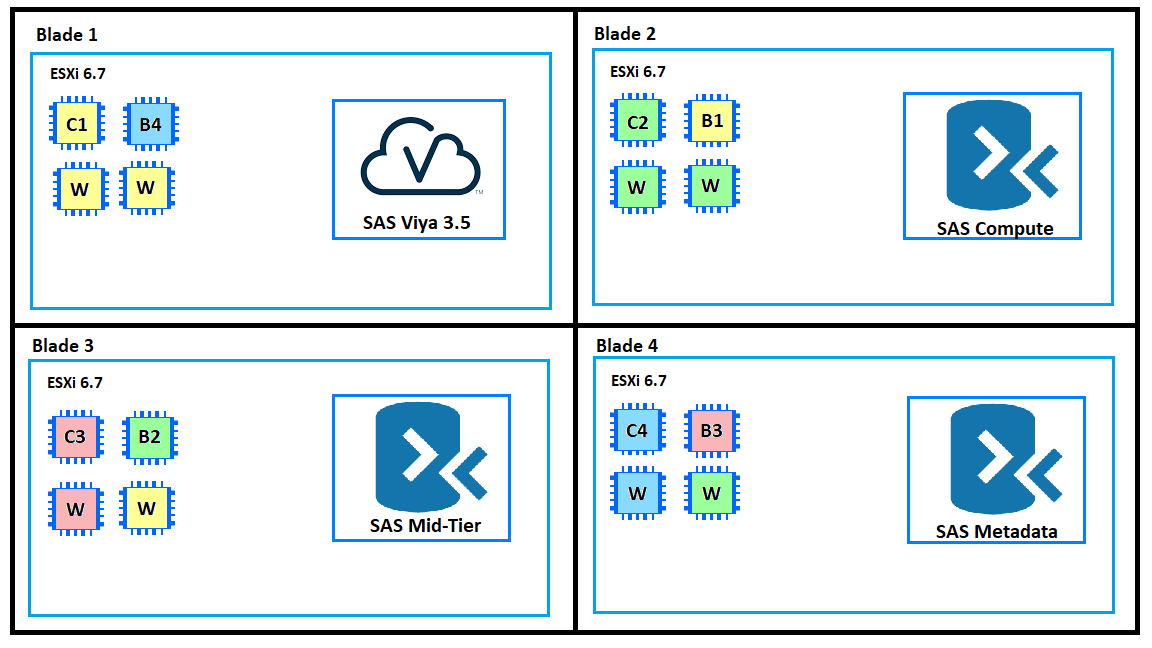
\includegraphics[scale = 0.52]{images/initial-deployment-diagram.png}
    \caption{Multi-Tenant Deployment (\textbf{Temporary Figure})}
    \label{Initial Multi-Tenant Deployment}
\end{figure} 

To maximize resource efficiency, CAS nodes will be evenly distributed across each blade, where a blade will consist of one controller, one backup controller, and two workers. The controller and backup controller, configured on the same system, will belong to separate tenants. The workers will also belong to separate tenants but each blade will have at least one related controller and worker per system. 

Subsequently, four additional VMs will be created to support the installation of SAS Viya 3.5 and SAS DMA. SAS Viya 3.5 will be installed as software on top of a RHEL 3.7X VM instance, in Blade 1. SAS DMA consists of three software components that will installed as software on top of Windows Server 2019 VM instances, in Blades' 2, 3, and 4. 

%----------------------------------------------------------------------------------%
\subsection{Implementation I}

The Implementation phase is a pivotal stage in deploying a robust SAS infrastructure following the SDLC framework. This phase involves executing the deployment plan, installing the selected hardware and software components, and configuring the system according to the defined technical specifications. Thorough testing and verification procedures are conducted to ensure the system functions as intended.

\begin{figure}[H]
    \begin{center}
        \renewcommand{\arraystretch}{1.5}
        \begin{tabular}{|>{\raggedright\arraybackslash}m{9cm}
                        |>{\raggedright\arraybackslash}l
                        |>{\raggedright\arraybackslash}l
                        |>{\raggedright\arraybackslash}l
                        |}
        \hline
        \rowcolor[HTML]{196fb4}\centering\textcolor{white}{\large Software} 
                                & \centering\textcolor{white}{\large Installed}
                                & \centering\textcolor{white}{\large Date}
                                & \centering\textcolor{white}{\large Status}
                                \tabularnewline 
        \hline
        SAS 9.4 & Completed & April 18, 2023 & Online\\\hline
        SAS Data Management Advanced Server & Completed & June 15, 2023 & Online\\\hline
        SAS Enterprise Guide & Completed & June 15, 2023 & Online\\\hline
        SAS/ACCESS to MS & Completed & June 15, 2023 & Online\\\hline
        \end{tabular}
    \end{center}
\caption{SAS 9.4 Installation Status}
\label{SAS 9.4 Installation Status}
\end{figure}

\begin{figure}[H]
    \begin{center}
        \renewcommand{\arraystretch}{1.5}
        \begin{tabular}{|>{\raggedright\arraybackslash}m{9cm}
                        |>{\raggedright\arraybackslash}l
                        |>{\raggedright\arraybackslash}l
                        |>{\raggedright\arraybackslash}l
                        |}
        \hline
        \rowcolor[HTML]{196fb4}\centering\textcolor{white}{\large Software} 
                                & \centering\textcolor{white}{\large Installed}
                                & \centering\textcolor{white}{\large Date}
                                & \centering\textcolor{white}{\large Status}
                                \tabularnewline 
        \hline
        SAS Visual Analytics & Pending & TBD, 2023 & Offline \\\hline
        SAS Visual Statistics & Pending & TBD, 2023 & Offline \\\hline
        SAS Visual Data Mining and Machine Learning & Pending & TBD, 2023 & Offline \\\hline
        SAS Visual Forecasting & Pending & TBD, 2023 & Offline \\\hline
        SAS In-Memory Statistics & Pending & TBD, 2023 & Offline \\\hline
        Viya Platform & Pending & TBD, 2023 & Offline \\\hline
        Visual Text Analytics & Pending & TBD, 2023 & Offline \\\hline
        Model Manager & Pending & TBD, 2023 & Offline \\\hline
        SAS Optimization & Pending & TBD, 2023 & Offline \\\hline
        SAS IML (Interactive Matrix Language) & Pending & TBD, 2023 & Offline \\\hline
        SAS QC (Quality Control) & Pending & TBD, 2023 & Offline \\\hline
        SAS Econometrics & Pending & TBD, 2023 & Offline \\\hline 
        Data Preparation & Pending & TBD, 2023 & Offline \\\hline
        SAS/ACCESS Engines & Pending & TBD, 2023 & Offline \\\hline
        Visual Analytics Add-In For Office & Pending & TBD, 2023 & Offline \\\hline
        \end{tabular}
    \end{center}
\caption{SAS Viya 3.5 Installation Status}
\label{SAS Viya 3.5 Installation Status}
\end{figure}

%----------------------------------------------------------------------------------%

\subsection{Testing \& Integration I}

During the Testing and Integration phase, comprehensive testing is performed to validate the functionality, performance, and reliability of the SAS infrastructure. Integration testing is carried out to ensure seamless interaction between different system components and to verify data integrity and accuracy. This phase also includes conducting user acceptance testing to ensure that the system meets the requirements and expectations of end-users.

To ensure the security of UHTASI's system and network, a comprehensive assessment will be conducted through a red team exercise, encompassing both vulnerability scanning and penetration testing. UHTASI will engage a trusted third-party organization (TTPO) to perform the assessment. This approach allows for an unbiased evaluation of UHTASI's security measures and helps identify any vulnerabilities that could be exploited by malicious actors.

\subsubsection{Rules of Engagement}
Define the scope, objectives, and limitations the TTPO must abide by during the assessment of UHTASI's system and network. As UHTASI handles sensitive PHI, it is crucial to adhere to these rules of engagement to ensure compliance with HIPAA and to avoid damage to data sources (Items listed below are sample rules and not actual limitations):

\begin{itemize}
    \item Avoid causing any damage or disruption to production systems.
    \item Exclude specific systems, networks, or assets from testing.
    \item Limit the scope to a specific set of vulnerabilities or attack vectors.
    \item Avoid testing third-party systems without proper authorization.
    \item Prohibit the use of Denial-of-Service (DoS) attacks or any actions that may impact system availability.
    \item Restrict testing to a specific environment or network segment.
    \item Exclude social engineering or physical penetration testing.
    \item Do not attempt to exploit known critical vulnerabilities without prior approval.
    \item Avoid any activities that violate local or international laws.
    \item Do not conduct the testing on live customer or user data.
\end{itemize}

\subsubsection{Reconnaissance}
\textbf{TBD}
\subsubsection{Scanning}
\textbf{TBD}
\subsubsection{Vulnerability Assessment}
\textbf{TBD}
\subsubsection{Exploitation}
\textbf{TBD}
\subsubsection{Analysis}
\textbf{TBD}
\subsubsection{Remediation}
\textbf{TBD}

%----------------------------------------------------------------------------------%

\subsection{Operations \& Maintenance I}

In the Operations and Maintenance phase, ongoing operational activities and system maintenance tasks are performed to ensure the smooth operation and longevity of the SAS infrastructure. This includes monitoring the system's performance, troubleshooting and resolving any issues, applying necessary updates and patches, and conducting regular backups and data management. Proactive maintenance and periodic system audits are conducted to optimize system performance, enhance security, and adhere to compliance standards.